\section{Introduction}
We will now consider scattering around two cylinders. To do this we first need to consider the relative positions of these two cylinders in relation to each other. To do this we consider their centers as their respective origins, $O_1$ and $O_2$, and the relative position vectors $r_1$ and $r_2$ from these origins to a point $P$. This is illustrated in \figref{fig:problem_3}, which is taken from the Cambridge Encyclopedia of Mathematics \parencite{martin06scattering}. \par
%
  \begin{figure} \centering
    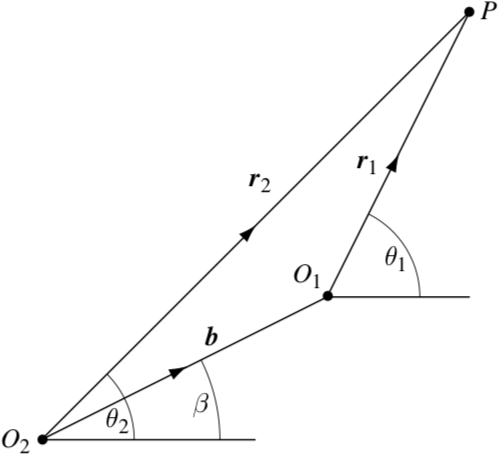
\includegraphics[width=6cm]{../figures/scattering_fig21.png}
    \caption{Multiple cylinder problem statement}\label{fig:problem_3}
  \end{figure}
%
  \begin{thm} \emph{Graf's addition theorem}. \par
    For $m \in \bb{Z}$:
      \begin{align*}
        J_m(kr_2)e^{im\theta_2} &= \sum^\infty_{n=-\infty} J_n (kb) e^{in\beta} J_{m-n} (kr_1) e^{i(m-n)\theta_1} \\
          & = \sum^\infty_{n=-\infty} J_{m-n} (kb) e^{i(m-n)\beta} J_n (kr_1) e^{in\theta_1}
        \end{align*}
  \end{thm}\par
%
Graf's original addition theorem gave an expansion for $J_\nu(kr)e^{i\nu\theta}$ where $\nu \in \bb{C}$, but we are only interested in $\nu \in \bb{Z}$, and this makes the proof simpler. The proof for this modified was allegedly first given by G.T. Walker in a now defunct journal called The Messenger of Mathematics, vol.25, of which it seems there are no digitalised copies! The proof is reproduced in the Cambridge Encyclopedia of Mathematics \parencite{martin06scattering}.
%
  \begin{proof} TBD, possibly omitted.
  \end{proof}
